\chapter[Statistical models for rates, ratios, and durations][Statistical models for rates]{Statistical models for rates, ratios, and durations}
\label{theory-rate_model}
\chapterprecis{Abraham D. Flaxman}

A central decision when modeling sparse, noisy epidemiological data
with Bayesian methods is the choice of the data likelihood function.
That is why the framework begins with a thorough discussion of the
alternative models for the meta-analysis of rates, ratios, and
durations.

A useful thought experiment to guide the development of
a metaregression technique is to consider how the model would proceed
if, for each and every study identified in systematic review, complete
microdata were available.  Of course, it is unusual that microdata are
available for even \emph{one} study from the systematic review.  However,
if all the microdata were available, say for all the prevalence
studies conducted on schizophrenia (an example I will return to in
the next section), modeling could proceed through standard techniques
for analyzing binary data, such as logistic or probit regression, with
fixed effects to explain some of the nonsampling variation, such as
differing diagnostic criteria, and random effects to model the
additional nonsampling variation, such as inherent differences
between populations (if they exist).

Viewed in this light, the task of a metaregression model is to
produce the results that would be obtained from an analysis of all the
microdata, if they were available. The approach that will be
developed below decomposes into three parts: the epidemiological rate
model, which captures the sampling error in systematic review data;
the age-interval model, which addresses the heterogeneity of age groups
reported in the literature; and the covariate model, which
models the nonsampling variation between different sources of data
through fixed and random effects.

The key to connecting the data for different epidemiological
parameters, such as incidence and prevalence, is the systems dynamics
model presented in chapter~\ref{theory-system_dynamics}.  This \emph{model of
  process} describes how the \emph{models of data} are related to each
other.  I will return to the model of process once the model of data
is fully developed.  The model of data is a statistical model that
has its core features defined by its likelihood function.  By
\emph{likelihood function}, I mean a probability density function that
assigns a value for the likelihood of every possible observed value
for any setting of the model parameters.

\section{A motivating example: Schizophrenia prevalence}
An example will make this clearer, so I turn now to the meta-analysis
of population prevalence of schizophrenia in adult males.  Strictly
speaking, prevalence is a ratio, although in the
literature the term ``prevalence rate'' is often used to mean
prevalence ratio.  The prevalence of a condition in a population says
something about the stocks in the stock-and-flow model from
chapter~\ref{theory-system_dynamics}: for a specific time period and
age group, prevalence is the ratio of individuals with the condition
to all individuals in the population.

The forest plot in figure~\ref{rate-model-schiz-forest} shows the
results of combining $16$ studies using $7$ different data models.  As
the figure demonstrates, the choice of data model can have a
substantial effect on the estimated uncertainty, and a
noticeable effect on the estimated median as well. The models I
display produce point estimates ranging from $1.2$ to $4.0$ per
$1000$ person-years and uncertainty intervals with widths ranging from $0.1$ to
$2.9$.  When analyzing sparse and noisy data, the choice of the data model
matters.

\begin{figure}[h]
\begin{center}
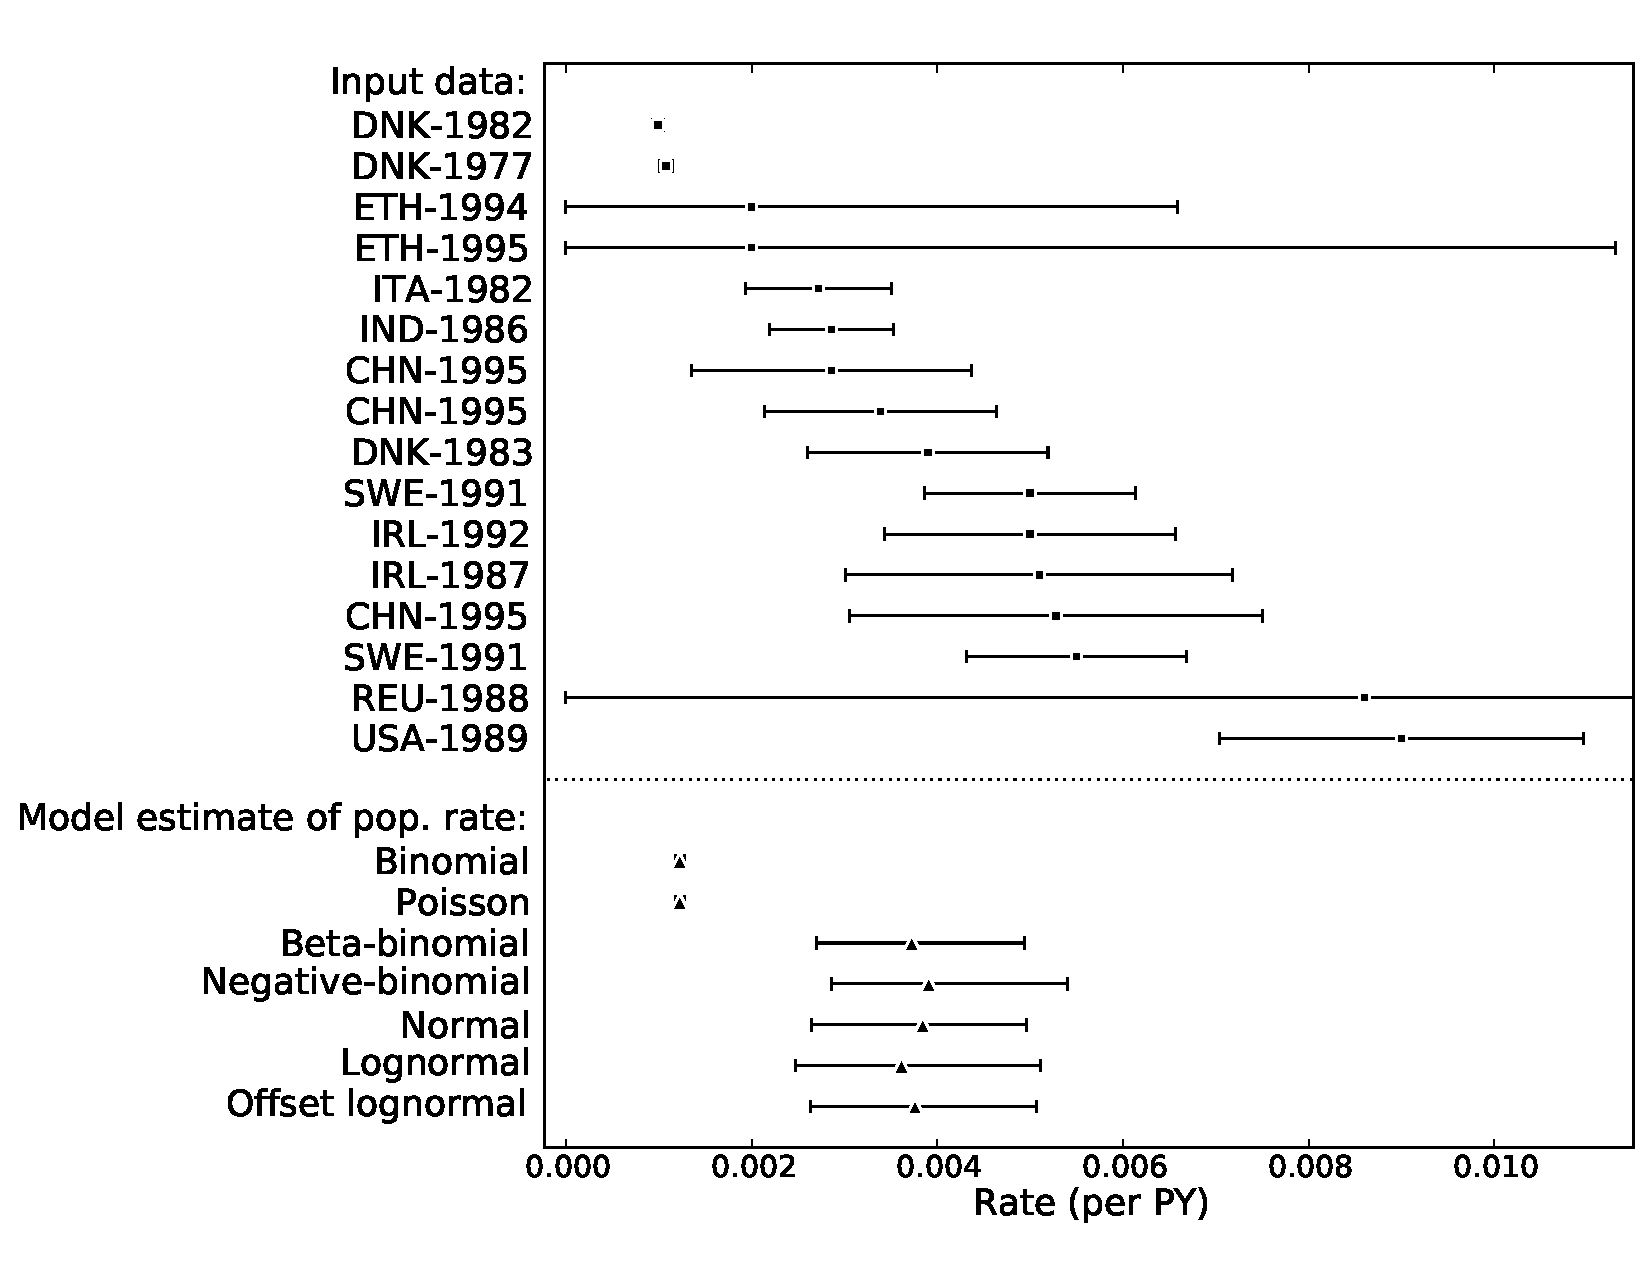
\includegraphics[width=\textwidth]{schiz_forest.pdf}
\caption[Forest plot of $7$ alternative models for meta-analysis of schizophrenia.]{Forest
  plot summarizing $7$ alternative models for
  meta-analysis of adult male schizophrenia prevalence at the
  population level.  The median estimates range from
  $1.2$ to
  $4.0$ per $1000$ person-years, and the width of the
  $95\%$ uncertainty interval ranges from
  $0.1$ to
  $2.9$.}
\label{rate-model-schiz-forest}
\end{center}
\end{figure}

In what follows, I will develop a collection of data models, starting
with the simplest and then increasing the complexity, while
identifying the benefits and drawbacks of each.  The models to come,
in order, are
\begin{itemize}
\item the binomial model,
\item the beta-binomial model,
\item the Poisson model,
\item the negative-binomial model,
\item three variants of the normal model,
\item the lower-bound data model.
\end{itemize}

\section{Binomial model}
Conceptually, the simplest model I consider for epidemiological data
is built from the binomial random variable. Random variable $X$ is
\emph{binomially distributed} if it has probability distribution
\[
\Pr[X=k\given n, \pi] = \binom{n}{k}\pi^k(1-\pi)^{n-k}
\]
for some $\pi$.  I have used Greek to emphasize that $\pi$ is a model
parameter, while $n$ and $k$ are data.

Although this equation may appear opaque, the intuition behind it is
simple: $n$ individuals were tested for a disease, and $k$ tested
positive. The formula then follows from the assumption that each
individual tested positive with probability $\pi$, and that if I know
$\pi$, then knowing about the test results of any subset of
individuals gives me no information about the test results for the
others (these events are ``independent'').

The intuitive description in the previous paragraph is particularly
relevant to a study that measures the \emph{prevalence} of a disease
in a population.  As mentioned above, prevalence is a \emph{ratio}, not
a rate.  It is a unitless metric, often expressed as a fraction or a
percentage.  Incidence, remission, and mortality rates, on the other
hand, are \emph{rates}, measured per unit time.  For example,
incidence is often expressed in the units of ``per person-year'' or
``per 1000 person-years.''  Nonetheless, the binomial distribution can
be the basis of a statistical model for rates as well as for
prevalence.  I will argue that it is not a very good model, and the
fact that, in its intuitive description, it may have the wrong units is
only one of its shortcomings.  It is instructive to
begin with simple models and make them more complicated until they
are just complicated enough.

The binomial distribution inspires a computationally tractable
data model for an observed population prevalence rate of
$r$ in a sample population of size $n$:
\[
\dens(r\given \pi, n) \propto \pi^{\lfloor rn \rfloor}(1-\pi)^{\lceil (1-r)n \rceil}.
\]
Here $\dens(\cdot)$ denotes a probability density function, $\lfloor
\cdot \rfloor$ is the ``floor'' operator, which rounds real numbers
down to the largest integer less than or equal to the operand, and
$\lceil \cdot \rceil$ is the ``ceiling'' operator, which rounds up.

Note that it is not necessary to include the normalization term
$\binom{n}{\lfloor np\rfloor}$, because this does not depend on the
model parameter $\pi$. This constant of proportionality is necessary
to make this data model truly a probability density function for any
$\pi$ and $n$. But I will never need to know this constant, and I use
the ``proportional to'' symbol $\propto$ instead of equality to
emphasize this fact.

In terms of the thought experiment from the introduction, this model
is equivalent to an analysis of all available microdata by fully
pooling all individual measurements from all studies.  It simply
uses the sample population from each study together with the rate to
find the number of positive observations.  In the parlance of
meta-analysis, this is a ``fixed-effect meta-analysis,'' because the
rate is modeled as fixed across all populations.\cite{borenstein_introduction_2011}

The funnel plot in figure~\ref{rate-model-binom-funnel} shows the
predictive distribution of this rate model for $\pi=.004$.  The
handful of square markers show the observed rate ($r$) and study size
($n$) from $16$ studies of schizophrenia prevalence. The more
plentiful circular markers are intended to give some idea of the shape
of the funnel predicted by the binomial rate model.  This figure shows
the potential problem with this approach: the data gathered by
systematic review are often much more dispersed than this distribution
predicts.  The binomial model row of the forest plot in
figure~\ref{rate-model-schiz-forest} shows the implications of this
problem in the case of schizophrenia prevalence: two large studies are
responsible for pulling the estimate below most of the observations,
while the pooled uncertainty interval is so small that it does not
overlap the uncertainty of most of the data points.


\begin{figure}[ht]
\begin{center}
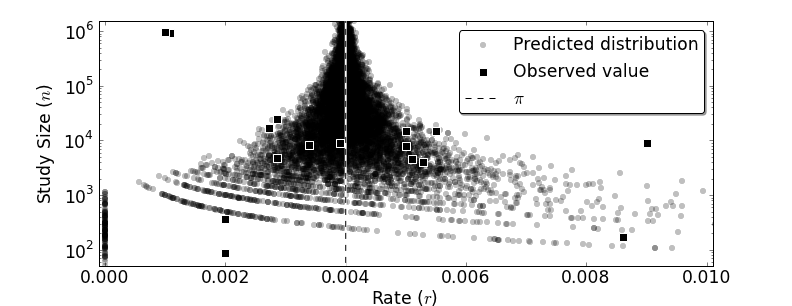
\includegraphics[width=\textwidth]{binomial-model-funnel.png}
\end{center}
\caption[Funnel plot for the binomial rate model.]{Funnel plot
  showing predictive distribution for the binomial
  rate model with $\pi=0.004$ (samples from this distribution are
  marked by circles), with data from systematic review for adult male
  schizophrenia prevalence overlaid for comparison (observations
  marked by squares).}
\label{rate-model-binom-funnel}
\end{figure}

There are two clear problems with this model---biased estimates and unreasonably high
confidence when modeling noisy data.  The model has small uncertainty intervals because it does not
account sufficiently for noise in the measurement of$ $r. If a study
of $50,000$ people from subpopulation A finds prevalence of $2$ per
$1000$ and a study of the same size in subpopulation B finds $6$ per
$1000$, then the binomial model predicts that a third study conducted
in subpopulation C will have prevalence of $4$ per $1000$, with an
uncertainty interval of $[3,5]$ per $1000$ (I use the 95\% highest
posterior density [HPD] interval as the uncertainty).  I have no
problem with the point estimate; picking the mean of the two
populations seems just right.  But the uncertainty interval lacks face
validity.  It would be much more reasonable to have an uncertainty
interval as large as $[1,7]$ instead of one as small as this.

Another way to quantify the mismatch between the binomial rate model
and the observed data is through the posterior predictive check, an
in-sample goodness-of-fit test that graphically compares the observed
data to the \emph{posterior predictive distribution}, which is to say
the model's prediction for what the data should be, after it has been
fitted to the data.\cite{gelman_bayesian_2003}
Figure~\ref{rate-model-binom-ppc} shows $1000$ draws from the
posterior predictive distribution for each of the data observations,
together with the observation itself.  The model predictions are
compressed, showing a cloud of predicted points that often does not
include the observation.  Trusting the results of such a model leads
to inappropriately high certainty about the nature of these noisy data.

\begin{figure}[ht]
\begin{center}
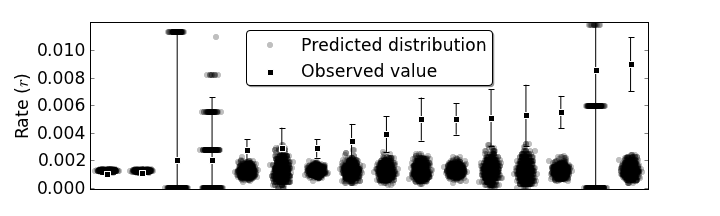
\includegraphics[width=\textwidth]{binomial-model-ppc.png}
\caption[Posterior predictive check for binomial model fitted to adult
  male schizophrenia data.]{Posterior predictive check for binomial model
  fitted to adult
  male schizophrenia data.  Circles show $1000$ draws from
  the posterior distribution of the binomial model, and squares
  show the observed data.  The uncertainty interval marked by error
  bars around each square shows the sampling error for each
  observation, based on the sample size alone. More than half of the
  data observations fall outside the posterior predictive distribution
  samples, indicating that the model is not capturing the
  heterogeneity observed in the data.}
\label{rate-model-binom-ppc}
\end{center}
\end{figure}


\section{Beta-binomial model}
\label{beta-binomial-model}
A theoretically appealing extension to the binomial model (which also
is not sufficient for my purposes) is the beta-binomial model.  I will
develop it in this section to motivate the following sections.

Formally, a beta-binomial random variable $X$ has the following
probability distribution:
\begin{align*}
\Pr[X = k\given n, \alpha, \beta]  &= \int_{\pi=0}^1 \dens(\pi\given \alpha, \beta) \binom{n}{k}\pi^k(1-\pi)^{n-k} \d\pi,\\
\dens(\pi\given \alpha, \beta) &\propto \pi^{\alpha-1}(1-\pi)^{\beta-1}.
\end{align*}

The intuition behind this model is simpler than the equation,
however. As in the binomial model, each individual tests positive for
the condition independently with a probability $\pi$, but now $\pi$
itself is a random variable, distributed according to a beta
distribution with parameters $\alpha$ and $\beta$. The beta
distribution is given by
\[
\dens(\pi\given \alpha, \beta)
\propto \pi^{\alpha-1}(1-\pi)^{\beta-1}
\]
and has a high degree of flexibility.  It always takes values
between $0$ and $1$, making it an appropriate distribution for a
probability.  Figure~\ref{rate-model-beta} shows the probability
density of the beta distribution for several combinations of $\alpha$
and $\beta$.
\begin{figure}[ht]
\begin{center}
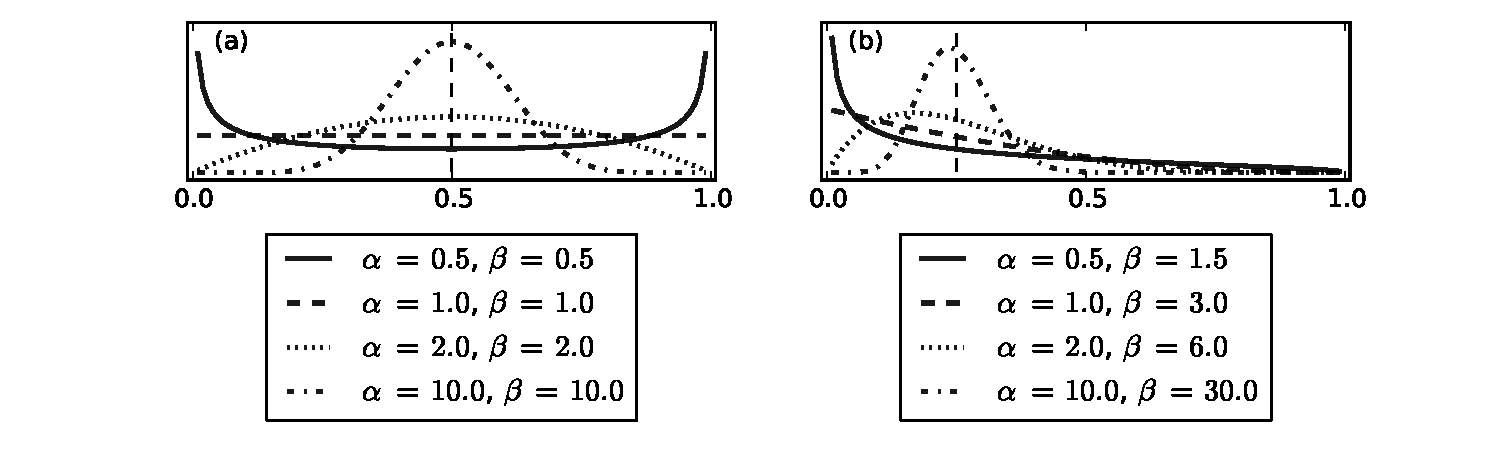
\includegraphics[width=\textwidth]{beta-distribution.pdf}
\end{center}
\caption[Probability density for the beta distribution.]{Probability
  density for the beta distribution for a range of
  $\alpha$ and $\beta$ values. The dashed vertical line shows the expected value,
  which is one-half for all distributions in panel~(a) and
  one-fourth for all in panel~(b).}
\label{rate-model-beta}
\end{figure}

The beta-binomial distribution inspires the following data model for
an observed rate of $r$ in a population of size $n$:
\[
\dens(r\given \alpha, \beta, n) \propto
\int_{\pi=0}^1 \pi^{\alpha-1}(1-\pi)^{\beta-1}
\pi^{\lfloor rn\rfloor} (1-\pi)^{\lceil (1-r)n\rceil} \d\pi.
\]

This model extends the binomial model in a way analogous to a random-effects
model in traditional meta-analysis\cite{borenstein_introduction_2011} (or in linear regression\cite{Rabe-Hesketh_Multilevel_2008}).  By introducing additional
dimensions into the parameter space, the model is able to capture the
dispersion beyond the binomial model that I have observed empirically
in funnel plots of real data.
Figure~\ref{rate-model-beta-binomial-funnel} shows the beta-binomial funnel
plot, as well as the posterior predictive check for
this model on the same data as used in
figure~\ref{rate-model-binom-ppc}.

\begin{figure}[ht]
\begin{center}
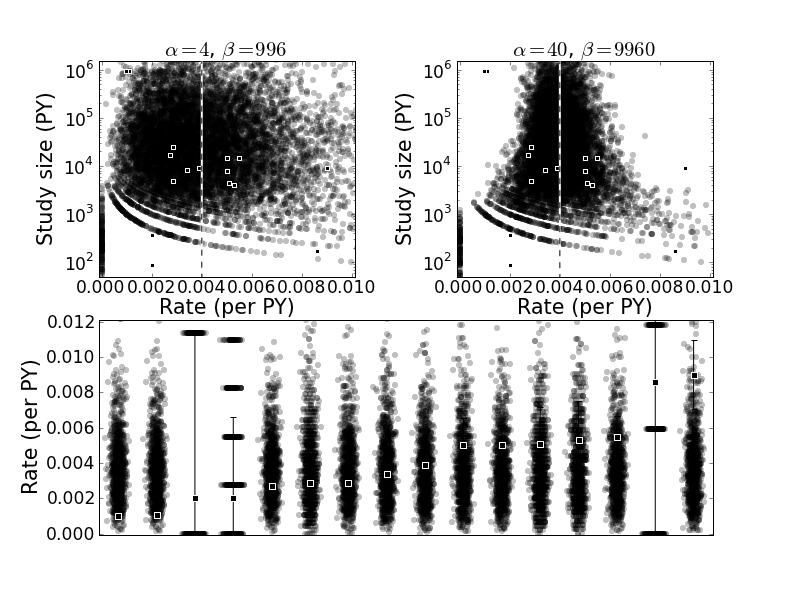
\includegraphics[width=\textwidth]{beta-binomial-funnel.png}
\end{center}
\caption[Funnel plots and posterior predictive check for the beta-binomial
  model.]{Funnel plots and posterior predictive check for the beta-binomial
  model. This model captures the heterogeneity in the observed data
  more faithfully than the binomial model from the previous section.
  However, the estimation procedure requires the introduction of a latent
  parameter for each data observation, and integrating out these
  latent variables is too computationally demanding to be feasible in
  many current applications.}
\label{rate-model-beta-binomial-funnel}
\end{figure}

This model addresses the theoretical shortcoming raised in the
previous section: if studies of $50,000$ people show prevalences of
$2$ and $6$ per $1000$, then the posterior distribution of the
beta-binomial model has mean $4$ with uncertainty interval $[1,8]$,
which seems quite reasonable.

The great shortcoming of the beta-binomial model is computational.
There is no closed-form solution to the integral in the probability
density for the beta-binomial model.  Evaluating it requires
introducing a latent variable for each of the data points in the
likelihood.  This simply takes too long to compute for the numerical
algorithms and computational infrastructure available in 2012.

\section{Poisson model}
There are two traditional approximations to the binomial distribution,
depending on how large $k$ is in relation to $n$.  When $k/n$ is
large, the normal distribution is used, and when $k/n$ is small, the
binomial is similar to the Poisson distribution.

Since I expect disease prevalence to usually fall in a ``small $k/n$''
setting, I will not develop the normal model in detail now, although
in section~\ref{transformed-normal-models} I will develop a model based on monotonic
transformations of the normal distribution that include a normal
model as a special case.

The Poisson distribution is given by the equation
\[
\Pr[X=k] =
\frac{\lambda^k e^{-\lambda}}{k!},
\]
and it can be understood intuitively as the number of times a
``memoryless'' event occurs in a unit time period.  Setting $\lambda
=\pi n$ produces an approximation to the binomial distribution that
is quite accurate for large $n$ and small
$k$. Figure~\ref{rate-model-poisson-approx-to-binom} demonstrates how
precise this approximation can be when approximating a binomial
distribution with $n=500$ and $\pi=\frac{1}{40}$.

\begin{figure}[h]
\begin{center}
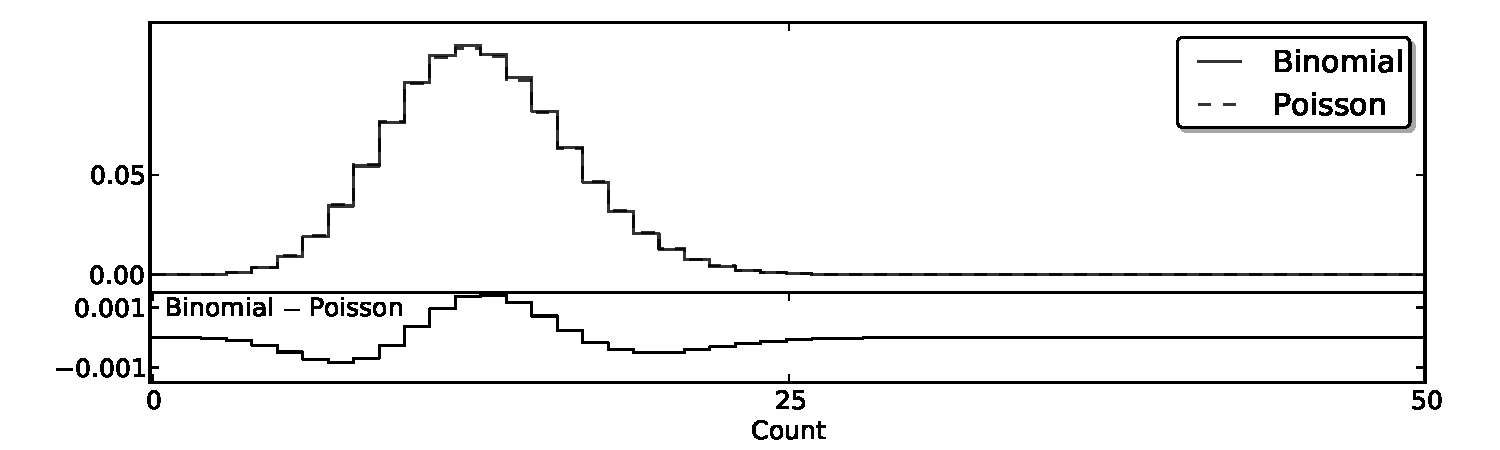
\includegraphics[width=\textwidth]{poisson_approx_to_binom.pdf}
\end{center}
\caption[The Poisson distribution approximates the binomial distribution 
  very closely.]{The Poisson distribution approximates the binomial
  distribution very closely. Here a binomial distribution with $n=500$
  and $\pi=1/40$ is approximated by a Poisson distribution
  with parameter $\lambda=25/2$.  The difference between the
  distributions is shown in the lower panel, since the curves in the
  upper panel are almost indistinguishable by eye.}
\label{rate-model-poisson-approx-to-binom}
\end{figure}

My Poisson rate model, which is defined from the Poisson distribution
in a manner analogous to the way the binomial distribution was
converted to a binomial rate model above, is the following:
\[
\dens(r\given \pi,n) \propto
(\pi n)^{\lfloor
  rn\rfloor} e^{-\pi n}.
\]
It is also subject to all of the concerns raised about the binomial
model.  When modeling rates with nonsampling variation at the level
typically found in systematic review, it will produce
inappropriately low estimates of uncertainty.

There is one key benefit to this model compared to the binomial and
beta-binomial models, however.  The Poisson model assigns a nonzero
likelihood to rates of more than $1$.  Although prevalence is always
less than $1$, it is theoretically possible to have incidence rates
more than $1$ (per person-year), and remission rates are often more
than $1$.  For prevalence, which, as discussed above, is actually a
unitless ratio of cases to population size, having nonzero probability
of values greater than $1$ is incorrect.  But for incidence,
remission, and excess mortality, which are measured per unit time,
having a model with a natural interpretation in the same units is
appealing.


\section{Negative-binomial model}
Another benefit from the count model approach is to be found in the
Poisson model's overdispersed cousin.  This distribution is called
the negative-binomial distribution (named after the formula that
proves it does indeed sum to $1$):
\[
\Pr[X = k\given \pi, \delta] =
 \frac{\Gamma(k+\delta)}{\Gamma(\delta)k!} \left(\frac{\delta}{\pi+\delta}\right)^\delta \left(\frac{\pi}{\pi+\delta}\right)^k.
\]
Unlike the beta-binomial distribution, it can be approximated
accurately without numerical integration.

However, this closed form obscures the intuition behind the
negative-binomial distribution, which is quite similar to the
intuition behind the beta-binomial distribution (but less clear from
its name). Through a bit of algebra, the negative-binomial
distribution can be represented as a hierarchical model where the
observed data come from a Poisson distribution, and the parameter of
the Poisson distribution is itself a random variable that comes from a
gamma distribution:
\begin{align*}
X\given \lambda &\sim \Poisson(\lambda),\\
\lambda &\sim \GammaDist(\pi, \delta).
\end{align*}

Here the gamma distribution is defined by
\[
\dens(\lambda \given \pi, \delta) \propto \lambda^{\delta-1} \exp\left(-\lambda \delta/\pi \right).
\]
The identity
\[
\frac{\Gamma(k+\delta)}{\Gamma(\delta)k!} \left(\frac{\delta}{\pi+\delta}\right)^\delta \left(\frac{\pi}{\pi+\delta}\right)^k
=
 C_{\pi, \delta} \int_0^\infty \frac{e^{-\lambda}\lambda^k}{k!} \lambda^{\delta-1} e^{-\lambda \delta/\pi} \d \lambda
\]
for an appropriate constant $C_{\pi,\delta}$ verifies this interpretation.

Through this lens, the negative-binomial model can be seen as a
natural adaptation of the traditional random effects model in linear
regression to the Poisson case, where each observation comes from a
different Poisson model and the Poisson parameters of these models are
all drawn from a common gamma distribution. Thus, a rate model based on
this distribution provides benefits in handling nonsampling variation
similar to those demonstrated for the beta-binomial distribution
above but in a formulation that is much less demanding
computationally.  The negative-binomial rate model for observing a
rate of $r$ in a population of size $n$ is
\[
\dens(r\given \pi, \delta, n) \propto
 \frac{\Gamma(\lfloor rn \rfloor+\delta)}{\Gamma(\delta)}
 \left(\frac{\delta}{\pi+\delta}\right)^\delta \left(\frac{\pi}{\pi+\delta}\right)^{\lfloor rn\rfloor}.
\]

Figure~\ref{rate-model-negative-binomial-funnel} shows funnel plots
for two levels of overdispersion, as well as the posterior predictive
distribution for the negative-binomial model.

\begin{figure}[h!]
\begin{center}
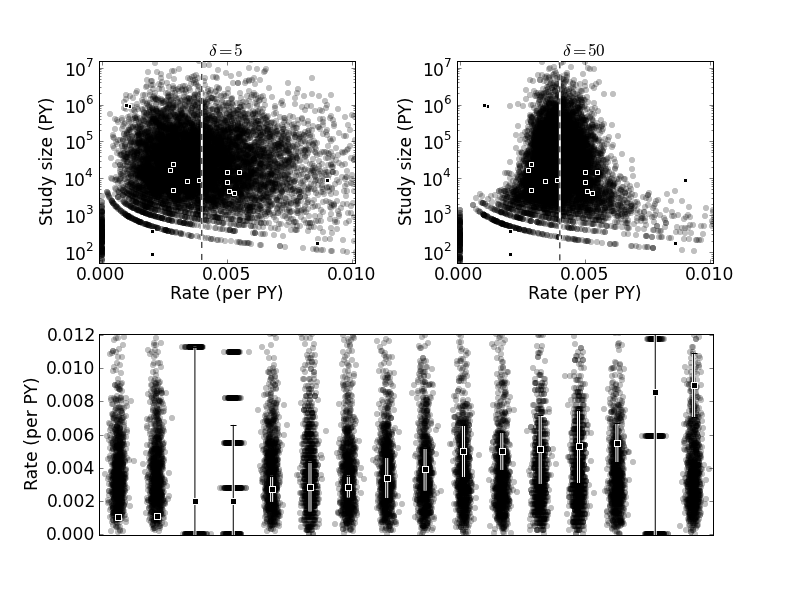
\includegraphics[width=\textwidth]{negative-binomial-funnel.png}
\end{center}
\caption[Funnel plots and posterior predictive check for the
  negative-binomial model.]{Funnel plots and posterior predictive check for the
  negative-binomial model. This model captures heterogeneity in
  observed data using an ``overdispersion'' parameter $\delta$ and
  can be interpreted as a hierarchical model, where each observation
  is drawn from a Poisson distribution that has its parameter drawn
  from a gamma distribution.  When $\delta$ is very large, the
  negative-binomial model is equivalent to the Poisson model.  The
  posterior predictive check shows that the uncertainty interval in the
  posterior predictions contains all the observed data, indicating
  that this model is sufficiently flexible to represent the observed
  heterogeneity.} \label{rate-model-negative-binomial-funnel}
\end{figure}

\section{Transformed normal models}
\label{transformed-normal-models}
Some epidemiological data are not related to count data at all.
Duration studies and studies measuring the relative risk of mortality
are two that come up frequently in systematic review.  For duration
data, a normal model is sufficient, and a lognormal model proves to
be appropriate for modeling relative risk data, which can be thought
of as a ratio of count variables.

Transformed normal models have also been used for mortality rates in
the
past\cite{girosi_demographic_2008,hogan_maternal_2010,rajaratnam_neonatal_2010}
and are worthy of continued consideration for modeling the incidence,
prevalence, remission, and mortality as an alternative to the
negative-binomial model.

In this section, I will develop a general transformed normal model
and compare it to the negative-binomial model.  The adjective
``transformed'' refers to a function that I will keep quite general
for now, only requiring it to be increasing and differentiable;
that is, for any $x > y$ the transformation $f$ must have $f(x) > f(y)$
and $f'(x)$ must be defined.  Then the transformed normal model will
be derived from the normal distribution, defined by the probability
density
\[
\dens(x\given \pi, \sigma)
 \propto \frac{1}{\sigma}
\exp\left\{ -\frac{(x-\pi)^2}{2\sigma^2} \right\}.
\]

For any increasing, differentiable function $f$, this distribution can
be converted to an $f$-transformed normal model with probability
density
\[
\dens(r \given \pi, \sigma, f, s) \propto
\exp\left\{-\frac{\left[f(r)-f(\pi)\right]^2}{2\left[(sf'(r))^2+\sigma^2\right]}\right\},
\]
where $s$ is the standard error of the rate $r$, which is more
convenient than the effective sample size $n$ in this case. The
denominator of the exponent deserves some additional discussion.  For
the identity function $f(x) = x$, the derivative $f'(x) = 1$, and the
denominator simplifies to $2(s^2 + \sigma^2)$, a familiar ``inverse
variance'' weighting, where $\sigma$ is a random effect to account for
overdispersion.  When $f$ is a more complicated function, the term
$sf'(r)$ approximates the standard error of the transformed value
$f(r)$.  Although more sophisticated approximations are possible,
experience dictates that the nonsampling variation (parametrized by
$\sigma$) is always larger than the chance variation, so a simple
approximation of the chance variation is sufficient.

Some common transformations of $f$ used in related work yield the
lognormal model $f(x) = \log x$, the logit model $f(x) = \logit(x)$,
and the probit model $f(x) = \probit(x)$.  All these approaches
have a significant drawback, however.  The transformation is not
defined for $x=0$, so these models cannot use data showing rates of
$0$. There are two common methods to fix this: dropping all $0$s
and adding a small offset.  Dropping measurements of $0$ is clearly
problematic, as it leads to systematic bias in the data that remain
and produces estimates larger than the truth.  This is especially
problematic for high-quality studies that focus on the age pattern of
a disease, where it is quite reasonable for some age groups to have
$0$ cases observed.  The effect of dropping $0$s is to overestimate
the rates in these age groups.

Adding a small offset, such as $0.5$, is an alternative solution,
and indeed, this is the approach taken for cause-specific mortality
estimation in a similar approach to mortality
modeling.\cite{girosi_demographic_2008} The selection of the offset
can seem ad hoc, however.

Within the framework of the transformed normal model, there is room to
put the solution on firm theoretical foundations.  For example, by
taking $f_\zeta(x) = \log(x + \zeta)$, I obtain the ``offset
log-transformed model,'' which does allow rates of $0$, simply by taking
a positive value for $\zeta$.  This model will not be used extensively
in the example application to come later in this book, but it seems
like a promising approach.  It is particularly appealing in the way it
decomposes the sampling variation into an additive error $\zeta$ and a
multiplicative error $\sigma$, and I expect that it will prove useful
in the future.  For completeness, here is the probability density for
the offset log-transformed model:
\[
\dens(r\given \pi, \sigma,\zeta, s)
\propto \exp\left\{
-\frac{\left[\log(r+\zeta)-\log(\pi+\zeta)\right]^2}
      {2\left[\left(\frac{s}{r+\zeta}\right)^2+\sigma^2\right]}
\right\}.
\]

\section{Lower-bound data model}
\label{theory-csmr}
Cause-specific mortality rates (CSMRs) are a special case among the
epidemiological rates available for integrative systems modeling of
disease in a population.  These data come from careful processing of
vital registration system outputs, from verbal autopsy studies, and
from some other sources. But when I introduce the compartmental model
of disease in a population in chapter~\ref{theory-system_dynamics},
there will be an important distinction about where CSMR data fit in.
Unlike incidence, prevalence, and remission data, they do not
correspond directly to any rate in the compartmental model.  This is
because of the operational requirement in vital registration systems
that each death have a single underlying cause.  The excess mortality
rate in the system dynamics model from
chapter~\ref{theory-system_dynamics} is not entirely compatible with
this idea.

In theory, the compartmental model could be extended to include CSMR
data explicitly simply by splitting the excess-mortality hazard $h_f$ flowing out
of the with-condition compartment $C$ into two parts.  These parts,
$h_{f'}$ and $h_{f''}$, would sum to $h_f$. The quantity $h_{f'}$ would denote the portion of
excess mortality caused directly by the disease, so any individuals
that exit compartment $C$ via the flow with hazard $h_{f'}$ would have this condition
listed as the underlying cause of death on their death certificate.
The quantity $h_{f''} = h_{f} - h_{f'}$ would then denote the ``excess excess mortality,''
which is to say the elevated mortality among individuals dying
\emph{with} the condition but not \emph{of} the condition.

Proceeding down this path promises to be extremely confusing!  It is
also a challenge because the sparse and noisy data available have
never been sufficient to separately estimate $h_{f'}$ and $h_{f''}$ with much
accuracy.  When the model is more flexible than the data, it is hard
to fit and the results are hard to interpret.

This motivates the alternative approach that I have taken, which
implicitly separates excess mortality into $h_{f'}$ and $h_{f''}$ but does
not try to explicitly represent both in the model.  It is a
``lower-bound'' likelihood, which contributes nothing to the likelihood as
long as the observation is below the prediction, and uses the Poisson
rate model when the observation is above the predicted level:
\[
\dens(r \given \pi,n) \propto
\begin{cases}
(\pi n)^{\lfloor rn\rfloor} e^{-\pi n}, &\qquad\text{if } \pi < r;\\
  0, &\qquad\text{otherwise.}
\end{cases}
\]

\section{Quantification of uncertainty}
The quantification of uncertainty in this metaregression challenge is
worthy of special attention.  The binomial, beta-binomial, Poisson,
and negative-binomial models developed above all rely on a
quantification of uncertainty in terms of persons or person-years,
denoted by $n$.  This is a stylized notion, however, based on a simple
model of the data generation process that uses a simple random sample.
In systematic review, it is common to find more complex survey
designs, and more sophisticated quantification of uncertainty is often
reported.  I call the corresponding $n$ the ``effective sample size,''
because it denotes the size that the sample would be if an identically
powered study \emph{did} use simple random sampling.

The transformed normal models above require a quantification of
uncertainty in terms of standard error, denoted by $s$.  Many studies
collected in systematic review report this value directly, but many
others do not.

It is useful to have a simple set of conversions to translate between
the $n$ needed for the count models, the standard error needed for the
transformed normal models, and the often-reported 95\% confidence
interval, which does not appear directly in any of the rate models
above. The approximate relationships between these quantities are
standard, and developing more precise transformations is not justified
due to the large amount of nonsampling variation in systematic review
data.

To represent a standard error $s$ in terms of a 95\% confidence
interval $(a,b)$, I have used the normal approximation
\[
s = \frac{b-a}{2\cdot 1.96}.
\]

To represent an effective sample size $n$ in terms of a standard error
$s$ and a observed rate $r$, I have two options.  For prevalence data,
where the standard error is for a ratio and hence constrained to be
between $0$ and $1$, I have used the binomial approximation
\[
n = \frac{r(1-r)}{s^2}.
\]
For other epidemiological rates, such as incidence and remission
rates, where the standard error is for a rate that is nonnegative but
could potentially be larger than $1$, I prefer the Poisson
approximation
\[
n = \frac{r}{s^2}.
\]

Some studies from systematic review report point estimates for
age-specific rates but quantification of uncertainty only at coarser
levels of aggregation, for example, only the sample size of the entire
study.  In these cases, I recommend a rough approximation that splits
the $n$ for the entire population among the subpopulations
proportionally to the population age structure.

Surprising as it may be, some studies from systematic review do not
report quantification of uncertainty at all.  It is often acceptable
to exclude these studies, and this exclusion criterion should ideally
be articulated at the beginning of the systematic review process.
Sometimes data are so sparse that it is not feasible to exclude studies
that do not quantify uncertainty, however.  In this case, I recommend
imputing the missing uncertainty interval (UI) values by taking them to have UI width equal to the $90$th
percentile value of the UI widths from the observations that do quantify
uncertainty.



\section{Summary and comparison}
This chapter has developed seven alternative rate models, all with
benefits and drawbacks.  The binomial model is simple and
theoretically appealing but does not handle nonsampling variation,
producing overconfident estimates in the face of noisy data.  The
beta-binomial model deals with overdispersion through a theoretically
appealing extension to the binomial model, but it is too
computationally demanding to use in my applications.  The Poisson
model is a close approximation to the binomial model and has all
the drawbacks except that it can handle rates greater than $1$, which is
important for modeling remission rates.  So it is the
negative-binomial model, which extends the Poisson model analogously
to the way the beta-binomial model extends the binomial model, that I
prefer on theoretical grounds.  This is the model that I have used for
most of the applications to follow, where it is applied to represent
data for incidence, prevalence, remission, excess mortality, and
cause-specific mortality. It is not as amenable to analysis as I would
like, however, and sometimes benefits from weakly informative priors on
the overdispersion parameter, an undesirable feature that slows down
analysis by requiring sensitivity analysis.  Transformed normal models
are a promising alternative approach, and I have used the normal model
for duration data in some of the following examples, as well as the
lognormal model for standardized mortality rate data and relative
mortality risk data. The offset log-transformed model seems
particularly promising as an alternative to the negative-binomial
model, and understanding its statistical and computational
characteristics is a promising direction for future research.  Like
the negative-binomial model, however, the convergence of these
transformed normal models also benefits from weakly informative priors,
a topic that deserves additional attention in the future.

Making a quantitative comparison of the models at this point is
challenging.  A simulation study depends critically on the
distribution used to simulate the data sets; so choosing a model 
that created the simulation data set will of course give promising 
results. A comparison based on out-of-sample predictive accuracy would be
preferable, but disease data are so sparse and noisy that such a comparison could be
meaningless, especially without including the adjustments for covariate
effects and age integration, which are developed in the next two
chapters.  A handful of diseases have data homogeneous enough in age
and geography to attempt a comparison of the models, but these are necessarily special
cases, and extending such findings to other settings must be done with
caution.  On the other hand, something is better than nothing.

To this end, I compared all models using a holdout cross-validation
approach.  I used this approach, described in
chapter~\ref{numerical-algorithms}, to generate $1000$ samples of the
model parameters from the joint posterior distribution for each model,
using random subsets of the data on epilepsy prevalence collected from
systematic review\cite{TK_Epilepsy_EG_report} in the model likelihood.  This data set
contains $1719$ observed prevalence values, and the level varies
little as a function of age, time, or geography.  I included each
observation in the subset to fit independently with probability $0.75$,
yielding a subset with around $1300$ observations. Then I fitted each
model with this subset and used the fit to predict values for the
observations that were not included in the subset.  I measured the
bias, median absolute error, coverage probability, and computation
time for each model and repeated this experiment $100$ times.  The
results are shown in table~\ref{rate-comparison}.

\begin{table}
\caption{Median results of holdout cross-validation of rate models
  for $100$ replicates for out-of-sample prediction.}
\label{rate-comparison}
\begin{center}
\begin{tabular}{|r|c|c|c|c|}
\hline
Rate Model       &Bias (\%)&MAE (\%)&PC (\%)&Time (s)\\
\hline
Binomial         &0.38     &0.26    &3.1    &110\\
Beta-binomial    &0.33     &0.26    &30     &190,000\\
Poisson          &0.38     &0.26    &3.1    &84\\
Negative-binomial&0.09     &0.36    &91     &170\\
Normal           &0.0009   &0.42    &95     &100\\
Lognormal       &-530     &230     &100    &140\\
Offset lognormal&0.0008   &0.42    &95     &140\\
\hline
\end{tabular}
\end{center}
\mynote{Bias is the mean
  of observed minus predicted, median absolute error (MAE) is the median of
  the absolute difference between observed and predicted, probability
  of coverage (PC) is the fraction of observed falling within $95\%$ uncertainty
  interval of prediction, and time is the computation time.}
\end{table}


  The beta-binomial
  model has coverage probability $10$ times higher than the binomial and Poisson models,
  which also minimize median absolute error, but takes $1000$ times
  longer to compute and is still far from the target probability of coverage of $95\%$.
  The lognormal model diverged for the majority of replicates, but
  with carefully chosen priors on overdispersion, it can be quite
  accurate.  In addition to being theoretically justified, the
  negative-binomial model has the superior balance of low median absolute error and high
  probability of coverage, with computation time only twice that of the fastest of the
  models.
